\documentclass[11pt]{amsart}
\usepackage[T1]{fontenc}
\usepackage{lmodern,amsmath,amssymb,amsthm,mathtools,booktabs,longtable,array,graphicx}
\usepackage[margin=1in]{geometry}
\usepackage{xcolor,enumitem,listings}
\usepackage[colorlinks=true,linkcolor=blue!45!black,citecolor=blue!45!black,urlcolor=blue!45!black]{hyperref}
\usepackage{microtype}
\newtheorem{theorem}{Theorem}[section]
\newtheorem{proposition}[theorem]{Proposition}
\newtheorem{lemma}[theorem]{Lemma}
\newtheorem{corollary}[theorem]{Corollary}
\theoremstyle{definition}\newtheorem{definition}[theorem]{Definition}
\newtheorem{example}[theorem]{Example}
\theoremstyle{remark}\newtheorem{remark}[theorem]{Remark}
\newcommand{\Z}{\mathbb Z}\newcommand{\N}{\mathbb N}
\newcommand{\MA}{\mathrm{MA}}\newcommand{\NMA}{\mathrm{NMA}}
\newcommand{\htq}{\operatorname{ht}}\newcommand{\Pf}{\operatorname{Pf}}
\newcommand{\pos}[1]{[#1]_+}\newcommand{\negp}[1]{[#1]_-}
\newcommand{\code}[1]{\texttt{\small\detokenize{#1}}}
\newcommand{\Ssix}{\mathcal S}\newcommand{\mut}[1]{\mu_{[#1]}}
\lstset{basicstyle=\ttfamily\small,breaklines=true,columns=fullflexible,keepspaces=true,frame=single}
\title[Mutation-acyclicity of four-vertex quivers]{Mutation-acyclicity of four-vertex quivers:\\a corrected classification, polynomial obstructions, and finite search}
\author{Kymani T. K. Armstrong-Williams}
\address{Centre for Theoretical Physics and Astronomy, Queen Mary University of London, London E1 4NS, United Kingdom}
\email{k.t.k.armstrong-williams@qmul.ac.uk}
\author{Edward Hirst}
\address{Institute of Mathematics, Statistics and Scientific Computing, University of Campinas (Unicamp), Campinas 13083-859, Brazil}
\email{ehirst@unicamp.br}
\author{Blake Jackson}
\address{Institute for Computer-Aided Reasoning in Mathematics, Carnegie Mellon University, 4720 Forbes Avenue, Pittsburgh, PA 15213, USA}
\email{blakej@andrew.cmu.edu}
\author{Kyu-Hwan Lee}
\address{Department of Mathematics, University of Connecticut, Storrs, CT 06269, USA; Korea Institute for Advanced Study, Seoul 02455, Republic of Korea}
\email{khlee@math.uconn.edu}
\date{9 October 2026. Internal research draft for author review.}
\keywords{quiver mutation, mutation-acyclicity, polynomial invariants, proper cyclic orders, computer-assisted proof}
\subjclass[2020]{13F60, 05E10, 68V15}
\begin{document}
\begin{abstract}
A quiver is mutation-acyclic if a finite sequence of mutations produces an acyclic quiver. We correct Theorem~2.9 of \emph{Machine learning mutation-acyclicity of quivers}: the double-arrow box is a counterexample to the asserted obstruction criterion. An exhaustive, independently reproducible classification gives a replacement: an input with arrow multiplicities at most two is mutation-acyclic exactly when it has an acyclicizing word of length at most three, with intermediate multiplicities at most two. We then exhibit an affine family whose nonnegative parameters alternate between the two mutation-acyclicity labels. Consequently no fixed finite Boolean combination of polynomial sign tests classifies all integral four-vertex quivers. A separate consequence of Chelnokov's invariant theorem, explicitly conditional on that external result, excludes chamberwise-polynomial invariants with arbitrary decoders under its hypotheses. Finally we give an input-dependent height bound, its excursion argument, and a deduplicated finite search algorithm. Exact arithmetic shortcuts substantially reduce search on a saved benchmark suite. We distinguish mathematical proofs, finite certificates, Lean checks, and measured performance.
\end{abstract}
\maketitle

\section{Introduction}
Quiver mutation is a local operation whose repeated application produces a rich global combinatorial structure. It arises in cluster algebras, representation theory and mathematical physics. An important question is whether a given quiver can be transformed into an acyclic one. Such a transformation allows methods developed for acyclic quivers to be applied throughout its mutation class. Finding a transformation proves a positive answer immediately; proving a negative answer requires control of all possible finite sequences.

Our previous paper \cite{AHJL} investigated this question for four vertices through computer-assisted classification and machine learning. Its polynomial support-vector-machine experiments also suggested looking for exact equations separating mutation-acyclic from non-mutation-acyclic quivers. Here we address the mathematical classification problem behind those experiments. We first correct an error in the stated bounded classification, then prove an obstruction to polynomial decision rules, and finally describe an exact algorithm with a finite stopping rule.

The error is in the characterization of the negative cases, rather than in the reported connected class counts. The double-arrow box is non-mutation-acyclic, but no member of its mutation class contains a non-mutation-acyclic full three-vertex subquiver. We give the missing mutation-class argument and replace the earlier theorem by a bounded-word criterion, supported by a complete census of $5^6$ labelled inputs.

The contrast with three vertices is sharp. In rank three, orientation and a cubic Markov expression give a finite polynomial-sign criterion. In rank four, the line
\[
 q(t)=(-2,t+2,t,-t,2-t,0)
\]
is mutation-acyclic for nonnegative even $t$ and non-mutation-acyclic for nonnegative odd $t$. Polynomial signs stabilize along an affine ray, whereas these labels do not. This proves an impossibility result without assuming a degree bound. Its proof uses the proper-order theorem of Neville \cite{Neville}, but neither the bounded census nor the height-bound theorem.

Impossibility in this language does not imply undecidability. We give a computable height $H(B)$ and prove that every mutation-acyclic input admits an acyclicizing path whose entire trajectory stays inside that height bound. A finite breadth-first search then decides the question. The proof must bound intermediate states, not just acyclic endpoints; the main work is an excursion reduction, including the signed identities in Appendix~\ref{app:excursion}. The algorithm combines this search with exact arithmetic criteria. Section~\ref{sec:experiments} reports new measurements of the supplied Python implementation; it contains no new machine-learning training experiment.

The bounded classification is computer-assisted. The proper-order results and the fork continuation result used below are external mathematical theorems, cited with their hypotheses. The invariant corollary has a further explicit dependency on Chelnokov's preprint. The finite-search correctness proof is mathematical, and relevant statements have a Lean realization. The Python implementation is independently checked, not extracted from Lean and not claimed to be formally verified.

\subsection{Conventions and preliminary results}
All vertices are mutable. Rank means the number of vertices, not the linear-algebraic rank of an exchange matrix. Thus singular matrices and disconnected quivers are included. We number the vertices $0,1,2,3$ and write
\begin{equation}\label{eq:matrix}
 B(q)=\begin{pmatrix}0&a&b&c\\-a&0&d&e\\-b&-d&0&f\\-c&-e&-f&0\end{pmatrix},
 \qquad q=(a,b,c,d,e,f)\in\Z^6.
\end{equation}
A positive $b_{ij}$ denotes $b_{ij}$ arrows $i\to j$. There are no loops or directed two-cycles. A directed adjacency matrix $A$ has nonnegative entries and $a_{ij}a_{ji}=0$; its exchange matrix is $B=A-A^{\mathsf T}$. Conversely $a_{ij}=\max(b_{ij},0)$. These two matrix conventions must not be confused.

Put $[x]_+=\max(x,0)$ and $\Delta(x,y)=[x]_+[y]_+-[-x]_+[-y]_+$. Mutation at $k$ is \cite{FZ}
\begin{equation}\label{eq:mutation}
 (\mu_kB)_{ij}=\begin{cases}-b_{ij},&i=k\text{ or }j=k,\\
 b_{ij}+\Delta(b_{ik},b_{kj}),&i,j\ne k.
 \end{cases}
\end{equation}
It preserves integrality and skew-symmetry and is involutive. A chronological mutation word $w=[k_1,\ldots,k_r]$ means $\mu_wB=\mu_{k_r}\cdots\mu_{k_1}B$. An \emph{acyclicizing word} has acyclic endpoint. We write $\MA(B)$ if such a word exists, including the empty word, and $\NMA(B)$ otherwise. A \emph{topological order} lists the vertices so that every arrow points forward. It exists exactly when the quiver is acyclic.

The \emph{support} is the undirected graph with edge $ij$ when $b_{ij}\ne0$. A full subquiver restricts to a subset of vertices and retains every arrow between them. Connectivity of support is mutation invariant: a two-step contribution cannot cross a component cut, and involutivity gives the converse. The \emph{height} is $\htq(B)=\max_{i<j}|b_{ij}|$. For a permutation $s$, write $(B^s)_{ij}=b_{s(i)s(j)}$. Relabelling and simultaneous arrow reversal commute with mutation after the corresponding change of mutation labels.

\begin{proposition}[Rank-three criterion and heredity]\label{prop:rank3}
For consecutive signed cycle entries $(x,y,z)=(b_{ij},b_{jk},b_{ki})$, set
\begin{align*}
 \mathcal T(x,y,z)\ \Longleftrightarrow\ &
 \bigl(x,y,z\ge2\ \land\ x^2+y^2+z^2-xyz\le4\bigr)\\
 &\lor\bigl(x,y,z\le-2\ \land\ x^2+y^2+z^2+xyz\le4\bigr).
\end{align*}
A three-vertex quiver is NMA exactly when $\mathcal T$ holds. A full subquiver of an MA quiver is MA.
\end{proposition}
The first assertion is the criterion of Beineke--Br\"ustle--Hille \cite[Theorems~1.1--1.2]{BBH}, expressed in signed coordinates. The second is \cite[Corollary~5.3]{BMR}, also proved in \cite[Proposition~2.3]{Warkentin11}. These are external inputs to the mathematical argument. In particular, on four vertices a sufficient NMA test is
\begin{equation}\label{eq:triangles}
 \mathcal T(a,d,-b)\lor\mathcal T(a,e,-c)\lor
 \mathcal T(b,f,-c)\lor\mathcal T(d,f,-e).
\end{equation}
For disconnected four-vertex inputs this is also necessary: every component has at most three vertices, mutation acts componentwise, and components with at most two vertices are acyclic.

\subsection{Proper cyclic orders and ordered scalars}\label{sec:proper}
We use the numbering of \cite[arXiv v3]{FN} and \cite[arXiv v2]{Neville}.
\begin{definition}\label{def:proper}
A \emph{cyclic order} lists the four vertices up to rotation. A vertex $k$ is \emph{proper} when every directed path $i\to k\to j$ occurs clockwise as $(i,k,j)$ \cite[Definition~5.2]{FN}. A \emph{wiggle} swaps cyclically adjacent vertices joined by no arrow \cite[Definition~2.3]{FN}. The resulting equivalence classes are \emph{wiggle classes}. A class is \emph{proper} if each vertex is proper in some representative of that class; the representative may depend on the vertex \cite[Definitions~5.4, 11.1]{FN}.
\end{definition}
\begin{definition}\label{def:transport}
To \emph{properly mutate} at $k$, choose a representative proper at $k$ and cut the circle there. In the remaining list the old outgoing neighbours precede the old incoming neighbours. Move $k$ clockwise past the outgoing neighbours, stopping before the incoming neighbours, and mutate the quiver. Non-neighbours may lie on either side of this cut; these choices give the same resulting wiggle class \cite[Definition~6.1]{FN}. A class is \emph{totally proper} if it and every class obtained by any finite succession of proper mutations are proper \cite[Definition~14.1]{FN}. Following an ordinary mutation word while updating this class is called \emph{proper transport}.
\end{definition}
Total properness allows every next vertex to be mutated: a proper representative at that vertex exists by definition. A full-support quiver has no wiggles, so its proper classes are exactly cyclic orders at which every vertex is proper.

There are six cyclic orders, represented by
$\Ssix=\{(0,s_1,s_2,s_3):(s_1,s_2,s_3)\text{ permutes }(1,2,3)\}$.
Define
\begin{align}
 P(q)&=af-be+cd, &\det B(q)&=P(q)^2,\label{eq:pf}\\
 M(q)&=a^2+b^2+c^2+d^2+e^2+f^2+abd+ace+bcf+def+acdf,\label{eq:scalar}\\
 M_s(B)&=M(q(B^s)).\nonumber
\end{align}
We call $M_s$ an \emph{ordered scalar}. The dependence on order matters. The scalars are constant on wiggle classes and under proper transport, being coefficients of the Alexander polynomial \cite[(9.6)--(9.7), Corollary~14.2]{FN}. In rank four this polynomial is determined by $M_s$ and $\det B$ \cite[Remark~9.4]{FN}. The unordered polynomial $M(q)$ is not a mutation invariant. For example, mutation at $2$ changes $(0,-1,0,1,0,0)$, of scalar $2$, to $(-1,1,0,-1,0,0)$, of scalar $4$.

\begin{lemma}[Endpoint bounds]\label{lem:endpoint}
If $B$ is MA and $s$ is a totally proper ordering, then
\begin{equation}\label{eq:endpoint}
 M_s(B)\ge0,\qquad 2|P(B)|\le M_s(B).
\end{equation}
For connected support, $M_s(B)\ge3$ and $2|P(B)|<M_s(B)$. An acyclic endpoint in a topological order has every coordinate at most $\lfloor\sqrt{M_s(B)}\rfloor$.
\end{lemma}
\begin{proof}
Neville's theorem gives a totally proper class for every MA quiver \cite[Theorem~1.1]{Neville}. Transport the supplied class along an acyclicizing word. At the endpoint, a topological ordering is totally proper by \cite[Remark~1.2]{Neville}. There is at most one totally proper class by \cite[Theorem~14.3]{FN}. Consequently the transported class is wiggle equivalent to a topological ordering, and its scalar equals the topological scalar. Merely being proper would not imply this step.

In topological coordinates all six entries are nonnegative. Thus
\[
 2|af-be+cd|\le2(af+be+cd)
 \le a^2+f^2+b^2+e^2+c^2+d^2\le M.
\]
Also each coordinate square is at most $M$. Connected integral support contributes at least three nonzero squares. Equality throughout the displayed inequalities forces $a=f$, $b=e$, $c=d$, all cubic and quartic terms to vanish, and no cancellation between the positive and negative Pfaffian terms. At most one of the pairs $(a,f),(b,e),(c,d)$ can then be nonzero, so the support is contained in a matching and is disconnected. Finally $|P|$ is mutation invariant (indeed $P(\mu_kB)=-P(B)$ in fixed labels), and proper transport preserves $M$. These facts transfer the bounds back to $B$.
\end{proof}

\section{The error in the bounded classification and its correction}\label{sec:correction}
The precise mathematical assertion of \cite[Theorem~2.9]{AHJL} was: if $Q$ has four vertices and arrow multiplicities in $\{0,1,2\}$, then $Q$ is NMA if and only if either its mutation class contains a quiver with an NMA full three-vertex subquiver, or $Q$ itself is isomorphic to the dreaded torus. This equivalence is false. Its numerical count of connected MA and NMA isomorphism classes remains correct.

\begin{proposition}\label{prop:box}
The double-arrow box $q_\square=(-2,0,2,-2,0,-2)$ is NMA, is not isomorphic to the dreaded torus, and no quiver in its mutation class has an NMA full three-vertex subquiver.
\end{proposition}
\begin{proof}
Its arrows form $1\to0\to3\to2\to1$, each with multiplicity two. Mutation at $0$ gives
\[
 C=(2,0,-2,-2,4,-2).
\]
Checking the six cyclic orders and their nonedge swaps gives exactly one proper class for $C$, represented by $(0,2,1,3)$; its ordered scalar is $0$. If $C$ were MA its totally proper class would be this class, contrary to the connected bound $M\ge3$ in Lemma~\ref{lem:endpoint}. This proves NMA. The dreaded torus displayed in \cite{AHJL} has full support (one double arrow and five single arrows), whereas $q_\square$ has four support edges.

For the assertion about the entire mutation class, use Warkentin's description of the alternating box with weights $a,b\ge2$ \cite[Example~6.11 and Lemma~6.7]{Warkentin14}. Its central quivers are the oriented box and its one-mutation images. Beyond these, the exchange graph is built from diamond regions and fork branches. We recall the inward argument, because the NMA label alone does not prove triangle avoidance.

In a fork, deletion of its return vertex is acyclic. In a diamond root the same holds for the return vertex; in a wing it holds for its inward special vertex. A tip has two inward special vertices, and both inward neighbours are wings of the same diamond. The transition rules in \cite[Definitions~6.3 and Lemmas~6.4, 6.7]{Warkentin14} build each new root or fork from an earlier parent, and each diamond in the order root, wings, tip. They cover every mutation, including returns.

Suppose that all full triangles at an earlier neighbour are MA. A triangle containing the inward mutation vertex is mutation equivalent, by that same mutation, to a triangle at the neighbour. A triangle omitting the vertex is the acyclic deletion just described. Thus the claim propagates to a root, wing or fork. At a tip every three-element set contains at least one of its two inward vertices, so the two earlier wings cover all four triangles. The central box has only acyclic triangles. Every triangle of a one-mutation image is either an unchanged deletion of the box or the mutation of one of its acyclic triangles. Induction on the recursive construction proves the claim for every descendant. Relabelling, arrow reversal, and different exchange-graph vertices representing the same quiver do not affect it. In particular the conclusion applies when $a=b=2$.
\end{proof}

\begin{theorem}[Corrected bounded classification; computer-assisted]\label{thm:census}
For every $q\in[-2,2]^6\cap\Z^6$, $B(q)$ is MA if and only if it has an acyclicizing word of length at most three. If it is MA, one can choose such a word with every prefix of height at most two. Up to vertex relabelling there are $667$ connected classes, of which $534$ are MA and $133$ NMA, and $28$ disconnected classes, of which $27$ are MA and one is NMA.
\end{theorem}
\begin{proof}[Finite certificate proof]
Enumerate all $5^6=15,625$ labelled tuples. Replace each by the lexicographically least of its $24$ vertex relabellings. This gives $695$ representatives; we do not identify mutations or global arrow reversals. For each representative enumerate the $85$ words of lengths zero through three, retaining positive witnesses whose entire paths have height at most two. This yields $561$ positive representatives. Their shortest retained witness lengths have distribution $425,118,16,2$ at lengths $0,1,2,3$ respectively.

The negative side is proved independently of failure of these short searches. Among connected representatives, $46$ have a word of length at most two leading to a triangle satisfying Proposition~\ref{prop:rank3}; $42$ already have that triangle. One further class has a closed labelled orbit of $24$ cyclic states (Appendix~\ref{app:finite}). The other $86$ have certificates excluding every initially proper class: either its scalar violates an endpoint condition, or a recorded sequence of at most four proper mutations reaches an improper class. Total properness and Lemma~\ref{lem:endpoint} justify these exclusions. The two finite scalar exclusions used here are verified below. The disconnected negative case is the Markov triangle and an isolated vertex. Every remaining representative has a checked positive word. These disjoint lists give the stated counts and both implications.

The supplied program \code{scripts/census.py} regenerates every representative and certificate, without importing any preassigned label or using the height theorem. The independent checker replays each certificate. The formal statement \code{corrected_bounded_classification} proves the same equivalence, bounded-prefix refinement, unique isomorphism census and counts. Its negative proofs use additional unbounded recursive regions; they are not a formalization of this particular $46/1/86$ certificate partition. The source map records that distinction.
\end{proof}

\section{Polynomial obstructions and the comparison with rank three}\label{sec:polynomial}
\subsection{An alternating affine family}
\begin{lemma}\label{lem:recurrence}
For every integer $t\ge0$, $\mut{0,1}B(q(t))=B(q(t+4))$.
\end{lemma}
\begin{proof}
Directly from \eqref{eq:mutation},
\begin{align*}
 \mu_0q(t)&=(2,-t-2,-t,t+4,t+2,0),\\
 \mu_1(2,-t-2,-t,t+4,t+2,0)&=(-2,t+6,t+4,-t-4,-t-2,0).
\end{align*}
Here we used $[t]_+=t$, $[-t]_+=0$, $[t+2]_+=t+2$, $[-(t+2)]_+=0$ and $[-(t+4)]_+=0$. In the second mutation the two contributions to the $23$ entry have opposite signs and both positive-part products vanish. These evaluations include $t=0$. They use $t\ge0$; this recurrence is not asserted for negative parameters.
\end{proof}

\begin{lemma}\label{lem:seeds}
The parameters $0,2$ give MA quivers; parameters $1,3$ give NMA quivers.
\end{lemma}
\begin{proof}
The positive arrows of $q(0)$ admit vertex ranks $(1,0,2,2)$. Mutation at $1$ sends $q(2)$ to $(2,0,2,2,0,0)$, with ranks $(0,1,2,1)$. Put
\[
 s_1=(-2,-1,-1,1,-1,1),\qquad s_3=(-2,1,-1,1,1,1).
\]
For each cyclic order the proper vertices are as follows, obtained by testing the directed two-step paths in Definition~\ref{def:proper}:
\begin{center}\begin{tabular}{ccc}\toprule
Order & $s_1$ & $s_3$\\\midrule
$(0,1,2,3)$ & $0,2,3$ & $1,2,3$\\
$(0,1,3,2)$ & $0$ & $1$\\
$(0,2,1,3)$ & $0$ & $0,1,3$\\
$(0,2,3,1)$ & $0,1,3$ & $0,1,2$\\
$(0,3,1,2)$ & $0,1,2$ & $1$\\
$(0,3,2,1)$ & $0$ & $1$\\\bottomrule
\end{tabular}\end{center}
Both quivers have full support, so every wiggle class is a singleton. No order makes all vertices proper. Neither seed can be totally proper, hence neither is MA by Neville's theorem. Finally,
\[
 \mut{0,1}s_1=q(1),\qquad \mut{1,0}q(3)=s_3.
\]
Mutation invariance gives the claimed negative labels. This proof makes no use of Theorem~\ref{thm:census} or of the finite search below.
\end{proof}

\begin{theorem}\label{thm:parity}
For $t\in\Z$, $\MA(q(t))$ holds exactly when $t<0$ or $t$ is even.
\end{theorem}
\begin{proof}
For $t\ge0$, apply Lemma~\ref{lem:recurrence} repeatedly and reduce modulo four, using Lemma~\ref{lem:seeds}. If $t\le-2$, ranks $(2,0,1,1)$ certify acyclicity directly; at $t=-1$ use $(2,0,3,1)$. Negative parameters are therefore handled directly, not by extending the recurrence.
\end{proof}
For $t=4n$ an explicit witness is $[1,0]^n$; for $t=4n+2$ append $[1]$. We do not claim these lengths are minimal for every $n$. Every $q(t)$ is connected: $01$ is always an edge, and each of $2,3$ is joined to at least one of $0,1$.

\subsection{No fixed polynomial-sign decision rule}
\begin{definition}
A \emph{polynomial-sign rule} is a finite Boolean combination of statements $p(q)=0$ or $p(q)>0$, where $p$ is a polynomial in the six entries with real coefficients. Strict or weak inequalities and their negations give the same language. The list of polynomials and the Boolean combination are fixed independently of the input.
\end{definition}
\begin{theorem}\label{thm:nogo}
No polynomial-sign rule decides MA on all integral four-vertex quivers, even if the domain is restricted to connected support.
\end{theorem}
\begin{proof}
Substitute $q(t)$ into each of the finitely many polynomials. The result is a univariate real polynomial. If it is identically zero, its sign is constant. Otherwise its sign is the sign of its leading coefficient for all sufficiently large positive $t$. Taking the maximum of finitely many thresholds shows that every atomic test, and hence their Boolean combination, is constant on the positive tail. But $q(4n)$ is MA and $q(4n+1)$ is NMA for arbitrarily large $n$. This contradicts Theorem~\ref{thm:parity}. Both are connected.
\end{proof}
The Lean theorem treats rational coefficients. The real-coefficient extension just proved is mathematical and is not claimed as a separate formal declaration.
\begin{corollary}
There is no uniform bound on the length of a shortest acyclicizing word for all four-vertex MA inputs.
\end{corollary}
\begin{proof}
For any fixed word, mutation is piecewise polynomial on a finite partition defined by polynomial signs. Acyclicity of the endpoint is the disjunction of its $24$ topological-order tests. A fixed length bound would therefore express MA as a finite disjunction of polynomial-sign rules, contradicting Theorem~\ref{thm:nogo}.
\end{proof}
A fixed polynomial-kernel SVM, or a fixed finite Boolean ensemble of polynomial tests, cannot be exact on all these inputs. This is a statement about the decision language, not a lower bound on error for a particular test distribution, and not a statement about all neural networks or algorithms.

\subsection{Mutation invariants with arbitrary decoders}\label{sec:invariants}
A polynomial-sign rule need not be mutation invariant. Conversely, an arbitrary decoder applied to an invariant need not be a polynomial-sign rule; for example a parity decoder is outside this language. The two obstructions must therefore be stated separately.

\begin{proposition}[External invariant dependency]\label{prop:invariant}
Assume Chelnokov's Theorem~1 \cite{Chelnokov}. Let $F$ be defined on real skew-symmetric $4\times4$ matrices, polynomial on each fixed-sign chamber, with compatible values on chamber boundaries, and invariant under every real matrix mutation. No map from the values of $F$ to $\{\MA,\NMA\}$ classifies all integral inputs. The same holds for any collection of such invariants.
\end{proposition}
\begin{proof}
The cited theorem gives $F(B)=f(\det B)$ for a univariate polynomial $f$. The acyclic tuple $(1,1,1,2,1,1)$ and the NMA finite-orbit tuple $(-2,1,1,-1,-1,-1)$ both have $P=2$ and determinant $4$. Hence all such invariant values agree, while their required labels differ.
\end{proof}
Chelnokov uses real matrices and the same positive-part mutation rule. We checked the proof beyond the abstract: it identifies chamber polynomials, then derives invariance along Pfaffian level sets. Degenerate parameters and the integer-only extension require care. We retain the explicit real-invariance hypothesis rather than assume that extension. The accessible record has only v1 (2023) and no journal reference. This external theorem is not part of our Lean verification; no assertion about arbitrary nonpolynomial invariants follows.

\subsection{Why rank three is different}
In rank three the signed orientation tests and the cubic expressions in Proposition~\ref{prop:rank3} are themselves a finite polynomial-sign classification. On a cyclic orientation, with positive edge magnitudes $x,y,z$, the Markov expression is $x^2+y^2+z^2-xyz$; the NMA condition also requires $x,y,z\ge2$. One must retain these extra conditions. A single scalar value alone does not classify all rank-three inputs: the cyclic $(2,2,2)$ and the acyclic single edge of weight two both have the usual Markov value $4$. Thus our comparison concerns the existence of a finite polynomial-sign decision rule, not an inaccurate claim that every label is determined by a bare scalar in rank three. The rank-four determinant collision is a different obstruction, with the additional external hypothesis in Proposition~\ref{prop:invariant}.

\section{An exact decision algorithm}\label{sec:algorithm}
\subsection{Arithmetic criteria used before search}
The following tests are partial: their failure to decide an input does not imply NMA.
\begin{proposition}\label{prop:five}
For positive integers $x,y,z,u,v$, the tuple $(0,-x,y,-z,-u,-v)$ is MA exactly when $xy\le v$.
\end{proposition}
\begin{proof}
Mutation at $0$ gives $(0,x,-y,-z,-u,xy-v)$. When $xy\le v$, the order $(3,0,2,1)$ is topological, including equality. Initially there is exactly one proper class, with representatives $(0,1,3,2)$ and $(0,3,2,1)$: the only nonedge is $01$, so these are joined by a wiggle, and testing the other four orders excludes them. In a representative proper at $0$, the old outgoing set is $\{3\}$ and the old incoming set is $\{2\}$. The rule of Definition~\ref{def:transport} moves $0$ past $3$ but not $2$, giving the class of $(0,2,1,3)$ after mutation. When $xy>v$, the directed path $2\to3\to1$ is a left turn. Its class is a singleton (the remaining nonedge $01$ is not adjacent in this cyclic order), so it is improper. The unique initial proper class is the only candidate for total properness and has now failed. Another proper class at the mutated quiver cannot repair this failure of transport. Neville's theorem proves NMA.
\end{proof}
\begin{proposition}\label{prop:positive}
The following are positive criteria with the indicated witnesses:
\begin{enumerate}[label=(\roman*)]
\item $(-1,-b,c,d,-1,0)$ with $b\ge0$, $c,d\ge1$, $d(c-1)\le b$, has witness $[1,3]$;
\item $(a,b,c,d,e,f)$ with $a<0$, $c,e>0$, $f<0$, $b\le cf$, $d\le ef$, has witness $[3]$.
\end{enumerate}
\end{proposition}
\begin{proof}
The respective endpoints are
\[
 (1,d(c-1)-b,1-c,0,-1,d),\qquad
 (a,b-cf,-c,d-ef,-e,-f).
\]
Topological orders are $(2,3,0,1)$ and $(2,3,1,0)$ respectively.
\end{proof}

For negative tests we enumerate the six cyclic orders, form their wiggle components, and retain the proper classes. If there are none, the input is NMA. If every proper class violates Lemma~\ref{lem:endpoint}, it is also NMA. Additionally neither ordered pair
\begin{equation}\label{eq:finiteexclusions}
 (M,P^2)=(11,16)\quad\hbox{or}\quad (18,49)
\end{equation}
can occur at a nonnegative topological endpoint. Each coordinate would be at most $\lfloor\sqrt M\rfloor$, so exhaustive substitution requires $4^6=4096$ and $5^6=15625$ tuples respectively; the saved checker finds no matching tuple. Rejecting every candidate proper class by these exclusions is sound by scalar transport. These particular exclusions are computer-assisted finite lemmas. Equality in $M=2|P|$ is already enough to reject connected support: $(0,0,2,-3,1,-1)$ has a unique proper class with $M=12=2|P|$.

\subsection{The bound on the entire path}\label{sec:height}
Define the input-computable integers
\begin{equation}\label{eq:budget}
 S(B)=\sum_{s\in\Ssix}|M_s(B)|,\quad
 H(B)=\sum_{i<j}|b_{ij}|+S(B),\quad N(B)=(2H(B)+1)^6.
\end{equation}
All six orders are used, including improper ones. This avoids an a priori choice of a totally proper class. The first summand ensures $\htq(B)\le H(B)$. Proper transport shows more: at any actual mutation descendant, in any relabelling or reversed frame, every supplied totally proper scalar is bounded in absolute value by $S(B)$. Indeed, transport it backwards along the actual word; it becomes one of the initial six scalars. The budget is not recomputed along the path. By Lemma~\ref{lem:endpoint}, every acyclic endpoint has height at most $S(B)$.

\begin{theorem}[Bounded acyclicizing paths]\label{thm:height}
If an integral four-vertex exchange matrix $B$ is MA, it has an acyclicizing word $w$ with $\htq(\mu_uB)\le H(B)$ for every prefix $u$ of $w$, including the empty prefix.
\end{theorem}
\begin{proof}
If the support is disconnected, its only possible cyclic component has three vertices. The rank-three descent of Proposition~\ref{prop:rank3} decreases the magnitude of its single changed edge at each step, so it never increases the height. This proves the assertion in that case. Assume henceforth that the support is connected.

Among all acyclicizing words choose one minimizing, in order: the maximum trajectory height $F$, the number of nonempty prefixes attaining $F$, and the word length. Three successive minima in $\N$ justify this choice; no algorithm for finding this minimum is assumed. If $F>H(B)$ put $T=F-1$. Both endpoints have height at most $T$. Choose an excursion from a state of height at most $T$ to its first return to that height range, whose intervening states have height $F$. Adjacent repeated letters can be deleted, so its first two pivots $i,j$ are distinct.

The local reductions of Appendix~\ref{app:excursion} apply with scalar ceiling $S(B)\le T$. A connecting edge of magnitude at least two forces every reduced continuation either to stay high or to exceed $F$, contradicting the return. A zero edge gives a commuting alternative route with the same labelled endpoint and no high state. A constant unit-pair block can be replaced by a route of length at most three inside the lower box, with an explicitly relabelled tail. Hence the only residual case has first three distinct pivots $[0,1,2]$, after relabelling and possible reversal, and low lead $(1,x,c,d,e,f)$.

The exhaustive sign split is $x<0<d$, $x<0,d\le0$, or $x\ge0$. The last two cases violate the scalar or Pfaffian bounds. In the first case the only remaining leads are
\[
 A_c=(1,-2,c,1,0,F-2c),\qquad
 I_{t,u}=(1,-1,-t,2,t-F,F-u),
\]
with $1\le c,t,u\le T$. The wall $t=u$ is excluded in Appendix~\ref{app:equal}. The first-return word for $A_c$ is $[0,1,2,0,2]$ and is replaced by $[1,0,2]$. For $I_{t,u}$ it is $[0,1,2]$, replaced by $[1,0,2,1,2]$ if $t>u$ and $[2,0,2,1,0]$ if $u>t$. The appendix gives all intermediate tuples and inequalities. Each replacement removes high states and has endpoint equal to the old endpoint up to a known permutation. Applying the inverse permutation to every subsequent pivot transports the entire tail, preserving all its heights and acyclicity. The resulting full word contradicts the second minimum, even when it is longer. Thus $F\le H(B)$.
\end{proof}
The appendix supplies the signed algebra and the exceptional-wall argument rather than referring to an inaccessible local manuscript. The formal assembly is \code{Rank4Classification.heightCoverage}; the source package retains the supporting lemmas.

\begin{corollary}\label{cor:wordbound}
Every MA input has an acyclicizing word of length at most $N(B)-1$ inside the height bound.
\end{corollary}
\begin{proof}
There are at most $N(B)$ labelled integer six-tuples of height at most $H(B)$. If a witnessing trajectory repeats a labelled state, delete the loop between its two occurrences. The suffix still starts at precisely the same state. Repeat until the path has no repeated state, giving at most $N(B)-1$ edges.
\end{proof}

\subsection{Pseudocode, correctness and resource limits}\label{sec:pseudocode}
The implemented order of tests is specified below. The finite-orbit table is checked once at module import. The double-box test mutates once and applies its proper-scalar certificate. On a disconnected positive input, the rank-three descent decreases the sum of edge magnitudes until the component becomes acyclic; the rank-three criterion guarantees a decreasing choice whenever a cyclic component is MA.
\begin{lstlisting}
CLASSIFY(A):
    validate A; set B = A - transpose(A)
    if B is acyclic: return MA with empty witness
    if a full triangle is NMA: return NMA with that triangle
    if B is disconnected:
        descend its MA triangle; return MA with the verified word
    if B is the double-arrow box: return NMA with its certificate
    if B lies on q(t): use the proved integer-parameter classification
    apply the five-parameter test and the two positive criteria
    if B belongs to the checked 24-state closed orbit: return NMA
    if every proper class fails an endpoint test: return NMA
    H = sum(abs(entries(B))) + sum(abs(M_s(B)) for the six orders s)
    queue = [B]; parent = {B: none}
    while queue is not empty:
        C = pop_front(queue)
        for k in [0,1,2,3]:
            D = mutate(C,k)
            if height(D) > H or D is in parent: continue
            parent[D] = (C,k)
            if D is acyclic:
                reconstruct and independently verify word; return MA
            push_back(queue,D)
    return NMA with exhausted-search certificate
\end{lstlisting}
For performance comparability the implementation computes $H$ before the tests, so its diagnostic bound is available even when a shortcut resolves the input. This changes no mathematical outcome. The search-only comparison skips the shortcuts but retains the initial acyclicity test and exactly the same search.

\begin{theorem}\label{thm:algorithm}
Without imposed resource limits, the algorithm terminates on every valid input and returns MA if and only if the input is mutation-acyclic. Its BFS expands each discovered labelled state at most once and evaluates at most $4N(B)$ candidate mutations.
\end{theorem}
\begin{proof}
Every shortcut is justified above; every positive shortcut returns a word checked by the mutation formula and a topological-order test. BFS stores a predecessor only on the first discovery of a state, so each queue entry is unique. All entries have height at most the fixed initial $H$; hence the queue can produce at most $N$ expansions. A found endpoint and its predecessor chain prove MA. Conversely, Theorem~\ref{thm:height} supplies a path inside this box whenever the input is MA. BFS visits every vertex reachable inside the box unless it finds an acyclic one first. Therefore exhaustion without one proves NMA. Each expansion tries four pivots, proving the bound.
\end{proof}
The $4N$ bound concerns the BFS branch, not all preliminary arithmetic or witness replay. Our double-box shortcut uses one mutation and does not enter BFS. Constructing the line witness uses $2\lfloor t/4\rfloor+(t\bmod4)/2$ mutations for nonnegative even $t$. Disconnected descent performs four candidates per strictly decreasing step, at most four times the initial sum of magnitudes. Independent witness verification is counted separately.

With $H$ fixed, a candidate mutation uses a constant number of operations on integers of $O(\log(H+1))$ bits, including temporary products of size $O(H^2)$. Thus the graph bound is an operation count, not a bit-complexity bound. Dictionary operations are expected-time operations in Python, and stored predecessors require $O(N\log(H+1))$ bits apart from object overhead. If the largest initial magnitude is $W$, then $H=O(W^4+W)$, so this estimate can be enormous as a function of input bit length. It is not a practical worst-case guarantee.

The diagnostic interface returns \code{UNKNOWN} on an imposed timeout or state cap. The simple \code{classify(adjacency)} interface returns \code{MA} or \code{NMA} on completion. Reaching a requested limit raises a \code{ResourceLimit} exception. A stopped search is never an NMA certificate. Exhausted-search negative certificates require redoing the exhaustive traversal; unlike positive words, they need not be compact.

\section{Numerical experiments}\label{sec:experiments}
The experiment is a fixed suite of 64 labelled inputs, with three repetitions per input and method (384 calls). We kept every generated input. The 28 named inputs comprise 14 examples chosen to exercise the stated branches and 14 parameters $t=-5,0,1,2,3,4,10,11,32,33,128,129,1000,1001$ of the alternating line. Using Python's pseudorandom generator with seed $20261009$, we also draw 24 independent six-tuples uniformly from $[-3,3]^6$. Finally, 12 planted MA inputs are obtained by drawing all six nonnegative topological entries uniformly from $\{0,1,2\}$ and applying six independent uniformly chosen mutations. The exact draws and generating words are saved.

Runs used an Apple M1 CPU (8 cores, 16 GiB RAM), macOS 26.3 on arm64, and CPython 3.9.6. The program is single-process. For each input the method order is hybrid/search, search/hybrid, hybrid/search. One acyclic warm-up call precedes measurement; there is no result cache. The finite-orbit table is built and checked at import. Each named call is capped at 100,000 discovered states or 3 seconds; each generated call at 25,000 states or 1 second. Timeouts are cooperative, checked once per BFS expansion (and during iterative witness construction). A state cap can therefore be reached before a time cap. Such runs return UNKNOWN.

Timing uses \code{perf_counter} inside the diagnostic call, including the calculation of $H$, tests, search and independent positive-witness replay. It excludes imports and file I/O. Discovered states and expanded states count only BFS states; shortcut-only calls report zero. Mutation evaluations count candidates in BFS, rank-three descent and iterative line reduction, including duplicate or out-of-box candidates. Fixed-word criteria construct their words directly. Witness replay mutations are a separate counter. These conventions explain, for example, why a positive fixed-word shortcut can have zero counted candidate mutations.

\begin{table}[htbp]\centering\scriptsize
\caption{Selected named inputs. Times are medians of three runs, in milliseconds. The full minimum/median/maximum values, expanded states and witness-replay counts are in the saved summary. $S$ and $E$ are discovered states and candidate mutations for search alone. A star means UNKNOWN at the state cap; the displayed time is time spent, not completion time. All hybrid calls in this table complete.}\label{tab:named}
\begin{tabular}{@{}lcrrrrrr@{}}\toprule
Input & Hybrid branch & $H$ & $\log_{10}N$ & Hybrid ms & Search ms & $S$ & $E$\\\midrule
Acyclic & acyc. & 59 & 12.5 & 0.026 & $0.025$ & 0 & 0 \\
Disconnected + & disc. & 109 & 14.0 & 0.113 & $0.114$ & 7 & 9 \\
Disconnected -- & tri. & 78 & 13.2 & 0.025 & $0.064$ & 2 & 8 \\
Double box & box & 72 & 13.0 & 0.182 & $14.341$ & 726 & 2,904 \\
Finite orbit & orbit & 59 & 12.5 & 0.028 & $0.464$ & 24 & 96 \\
$s_1$ & proper & 71 & 12.9 & 0.090 & $440.812$ & 22,896 & 91,584 \\
$s_3$ & proper & 71 & 12.9 & 0.101 & $439.053$ & 22,896 & 91,584 \\
Five + & five & 362 & 17.2 & 0.044 & $0.048$ & 2 & 1 \\
Five -- & five & 295 & 16.6 & 0.038 & $1996.809$ & 89,856 & 359,424 \\
Product & prod. & 439 & 17.7 & 0.056 & $0.147$ & 11 & 12 \\
Quadratic & quad. & 442 & 17.7 & 0.046 & $0.072$ & 5 & 4 \\
Scalar equality & proper & 97 & 13.7 & 0.186 & $270.536$ & 13,020 & 52,080 \\
Search positive & BFS & 80 & 13.2 & 0.191 & $0.058$ & 4 & 3 \\
$q(10)$ & line & 20,066 & 27.6 & 0.081 & $1.397$ & 102 & 234 \\
$q(11)$ & line & 29,352 & 28.6 & 0.031 & $1513.910^{*}$ & 100,000 & 284,309 \\
$q(128)$ & line & 536,871,450 & 54.2 & 0.548 & $77.486$ & 4,093 & 15,449 \\
$q(129)$ & line & 553,846,304 & 54.3 & 0.038 & $1228.819^{*}$ & 100,000 & 205,593 \\
$q(1000)$ & line & 2,000,000,004,026 & 75.6 & 3.840 & $712.278$ & 33,619 & 131,933 \\
$q(1001)$ & line & 2,008,012,012,032 & 75.6 & 0.043 & $1557.634^{*}$ & 100,000 & 281,707 \\
\bottomrule\end{tabular}\end{table}
The branch abbreviations denote acyclicity, disconnected descent, a rank-three obstruction, the double-box certificate, the finite closed orbit, proper-order exclusion, the line formula, the five-parameter criterion, the product and quadratic criteria, and bounded BFS, respectively. Every reported MA witness was also replayed after the experiment with a separate dense-matrix implementation. Completed labels agree between methods.

\begin{table}[htbp]\centering\small
\caption{All inputs, aggregated by sample. Time is the median of the three sums over the sample, in seconds. State and mutation columns sum the per-input medians. UNKNOWN calls are retained.}\label{tab:generated}
\begin{tabular}{llrrrrrr}\toprule
Sample & Method & MA & NMA & Unknown & Time (s) & States & Mutations\\\midrule
Named & hybrid & 15 & 13 & 0 & 0.0063 & 4 & 600 \\
Named & search & 15 & 9 & 4 & 12.9275 & 710,931 & 2,234,099 \\
Uniform & hybrid & 16 & 8 & 0 & 0.6070 & 30,146 & 120,538 \\
Uniform & search & 16 & 7 & 1 & 1.5973 & 77,946 & 309,310 \\
Planted & hybrid & 12 & 0 & 0 & 0.0051 & 299 & 606 \\
Planted & search & 12 & 0 & 0 & 0.0042 & 299 & 606 \\
\bottomrule\end{tabular}\end{table}

The hybrid method resolves all 64 inputs under these limits. Search alone resolves 59; four named inputs and one uniform draw reach their state caps in all repetitions. All 12 planted inputs are confirmed MA by both methods. This sample is small and deliberately includes structured cases; it is not an estimate of the proportion of MA quivers or of average complexity under a canonical distribution.

The contrast is especially clear for the two negative seeds: each has 22,896 states in its reachable height-bounded component, whereas the hybrid proof only inspects its six cyclic orders. For $q(1000)$ the line witness has 500 mutations and must be constructed and checked; its running time consequently grows with the witness length. The odd-line negative certificate does not construct such a trajectory. This is a difference in output work as well as search avoidance. The a priori state bound remains vastly larger than the explored components, including on inputs where BFS is required. It proves termination but is a poor practical predictor of runtime.

\begin{figure}[htbp]\centering
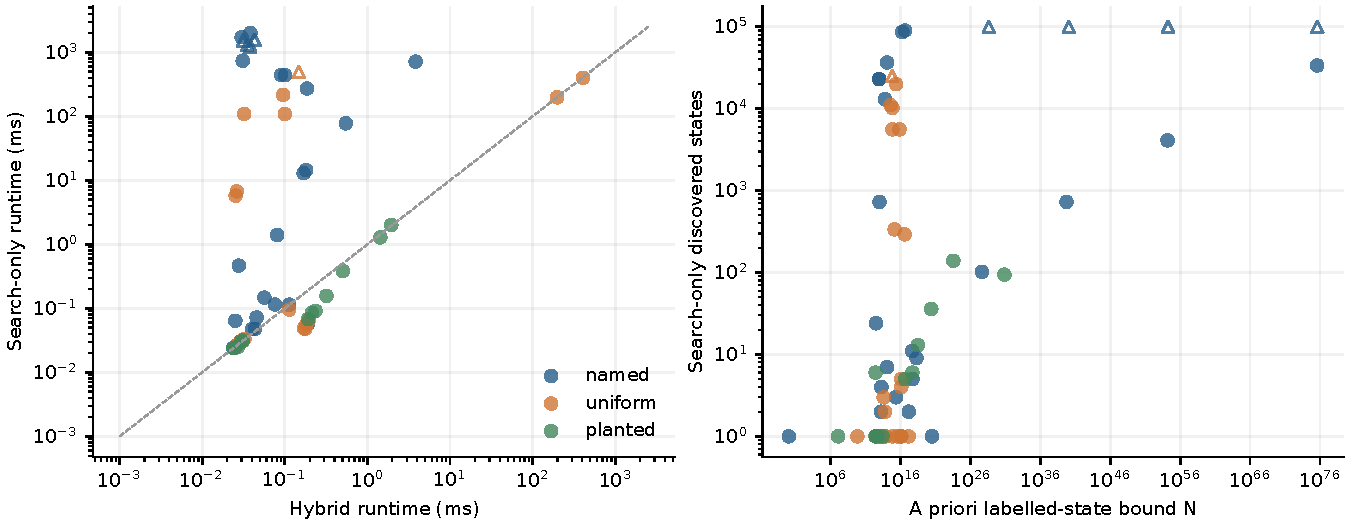
\includegraphics[width=\textwidth]{figures/performance.pdf}
\caption{Each marker represents one of the 64 inputs (medians of three calls). Left: paired runtimes; open upward triangles denote capped search-only runs and must not be read as completion times. The diagonal marks equal time. Right: discovered search-only states versus the labelled bound $N$; capped runs are open triangles. An initially acyclic input has zero BFS states, displayed here at one solely for the logarithmic axis.}\label{fig:performance}
\end{figure}
The plotting environment uses Python 3.12.14 and Matplotlib 3.10.7; its dependency lock is separate from the standard-library-only classifier. Tables and the figure are generated from the saved raw measurements, not from timings in the review report.


\section{Conclusion and reproducibility}\label{sec:conclusion}
The corrected bounded theorem preserves the previous connected counts while replacing an invalid characterization of the negative cases. The alternating family explains why a fixed collection of polynomial signs cannot give an exact rank-four rule, despite successful approximate classifiers on finite datasets. The finite-height theorem supplies a different type of classification: an input-dependent search with a mathematical stopping rule. Arithmetic certificates can make that search much smaller in practice, but the present experiments do not establish a practical worst-case bound or an arithmetic-only classification on every input.

The companion package contains the source manuscript, exact classifier, all benchmark inputs and raw measurements, scripts regenerating the tables and figure, and the selected Lean source closure. The private repository is \url{https://github.com/KTKAW/rank4-paper}; access requires permission from its owner. \IfFileExists{revision.tex}{\input{revision.tex}}{The draft source commit is recorded with the release bundle.}
 The Overleaf bundle is an upload-ready copy of the tested manuscript sources. No public archival identifier is claimed for this private draft.

Lean uses version 4.24.0 and the mathlib revision recorded in the locked manifest. Fresh checks and reused dependency objects are separated in Appendix~\ref{app:formal} and in the reproduction guide. The human proofs of the alternating family use the proper-order seed certificates; their revised Lean counterparts also avoid bounded-classification imports. The current Python classifier implements the deduplicated-state algorithm proved here. The older formal fallback enumerates words; the later formal frontier search proves the corresponding deduplicated-state semantics. None of these facts identifies Python bytecode with a Lean executable.

\appendix
\section{The excursion reduction in detail}\label{app:excursion}
This appendix contains the local algebra used in Theorem~\ref{thm:height}. Its hypotheses are essential: the matrices are actual prefixes of an MA input, and the scalar ceiling is inherited from that input. An arbitrary proper ordering or an arbitrary path between two small endpoints would not suffice.

The disconnected case was disposed of in the proof of Theorem~\ref{thm:height}; throughout this appendix the support is connected.

Throughout $T\ge H(B)$, $F=T+1$, and a state is called \emph{low} if its height is at most $T$, and \emph{high} if its height is $F$. These terms are used only in this appendix. All trajectory states under consideration have height at most $F$. At every actual prefix and in every signed permutation frame, every totally proper scalar $m$ satisfies
\begin{equation}\label{eq:prefixscalar}
 0\le 2|P|\le m\le S(B)\le T.
\end{equation}
For connected support, $m\ge3$ and $2|P|<m$. To obtain the assertion for a supplied totally proper ordering at a prefix, transport it along the reverse of that prefix to the input. Relabelling transports the pivot letters and global arrow reversal reverses the cyclic order. The resulting scalar is one of the six in $S(B)$.

\subsection{A strong first pair cannot return}
\begin{lemma}\label{lem:strong}
Let $P$ be an actual framed prefix. Suppose $\htq(P)=F$, $\htq(\mu_iP)\le T$, $\htq(\mu_jP)\le F$, $i\ne j$, and $|p_{ij}|\ge2$. No reduced word starting with $j$, and staying under the ceiling $F$, can reach a low state. Here reduced means that consecutive letters differ.
\end{lemma}
\begin{proof}
Put $i,j$ in positions $0,1$. Every entry incident to this pair is below $F$. For example, after orienting $p_{01}>0$, an entry $p_{12}=F$ which decreases under mutation at $0$ requires $p_{02}>0$; mutation at $1$ then creates $p_{02}+p_{01}F>F$. The negative wall and the other incident entries follow by reversal or exchange of the two remaining vertices. The sole possible top entry is therefore $23$. Reversal and exchanging $2,3$ put the state in the form
\[
 P=(a,b,-c,d,E,F),\qquad a\ge2,\quad b,c>0.
\]
The low child and the other ceiling give $b<F$, $ac-E<F$, and $b+ad\le F$ when $d\ge0$. A totally proper scalar $m$ exists and satisfies \eqref{eq:prefixscalar}, with Pfaffian $aF-bE-cd$.

We claim $d\ge0$ and $E\ge c$. If $d<0$, then $E>0$ creates $23$ entry $F+(-d)E>F$ under mutation at $1$, while $E\le0$ gives $P\ge2F$. If $d=0,E<0$ the same Pfaffian contradiction applies. The remaining two excluded chambers have a unique proper class (including its wiggles when a coordinate is zero), and its scalar is the following polynomial:
\begin{align*}
 K={}&a^2+b^2+c^2+d^2+E^2+abd-acE
       +F\{F-bc-d(ac-E)\} &&(0\le E<c),\\
 K_+={}&a^2+b^2+c^2+d^2+e^2+abd+ace
       +F\{F-bc-d(e+ac)\} &&(E=-e<0,d>0).
\end{align*}
Here is the arithmetic exclusion, retaining the guards needed in each case. In the first row suppose $0\le K\le F$ and $2|aF-bE-cd|\le K$. Set $x=b+(a-1)d$ and $y=c-E$. The height inequalities give $1\le x,y\le F-1$. The maximum of $x^2+y^2-Fxy$ on this integer rectangle is attained on its boundary, and is at most $2-F$ (fix one variable and use convexity, then repeat). Writing $p=aF-bE-cd$, the exact identity is
\[
 K=a^2+x^2+y^2-Fxy-(a-1)F^2+Fp
 -(a-2)\{d(b+ad)+cE+FdE\}.
\]
The braced term is nonnegative. Applying the rectangle bound and $2p\le F$ gives
\[
 2K\le2a^2+4-2F-(2a-3)F^2<0.
\]
For $a=2$ use $F\ge3$; for $a\ge3$ use $F>a$, which follows since $a$ is an incident entry. In the second row $e+ac<F$ and $b+(a-1)d<F$. Put $p=aF+be-cd$. Direct expansion gives
\[
 K_+=a^2+(b^2+d^2+abd)+(c^2+e^2+ace)
 -(a^2-1)F^2+apF-F(bc+de+abe).
\]
The two quadratic groups are bounded by $(b+(a-1)d)^2$ and $(ac+e)^2$, respectively, hence by $(F-1)^2$ each. Dropping the last nonpositive term and using $2p\le F$ gives
\[
 2K_+\le-(2a^2-a-6)F^2+2a^2-8F+4<0.
\]
For $a=2$ the last expression is $12-8F<0$; for $a\ge3$ its quadratic term is negative. Both contradict \eqref{eq:prefixscalar}. Thus $d\ge0,E\ge c$.

The next state is
\begin{equation}\label{eq:strongnext}
 \mu_1P=(-a,b+ad,-c+aE,-d,-E,F).
\end{equation}
Mutation at $2$ creates $03$ entry $-c+aE+(b+ad)F>F$. Mutation at $3$ exceeds the ceiling unless $d=0,E=c=1$. On that exceptional wall the proper scalar is
$m=a^2+b^2+F^2-a-bF+2>F$; this follows from
$b^2-bF\ge-F^2/4$, $a\ge2$, and $F\ge3$. Therefore reducedness forces the next pivot to be $0$.

The two columns at the remaining vertices are now aligned: in the orientation where the connecting edge is positive, one pivot row is nonpositive, the other nonnegative, and the latter dominates in absolute value. If $C_{i\ell}\le0\le C_{j\ell}$, $-C_{i\ell}\le C_{j\ell}$ and $C_{ij}\ge2$, mutation at $j$ replaces the entries by $C_{i\ell}+C_{ij}C_{j\ell}$ and $-C_{j\ell}$, preserving dominance. After one further pair mutation both signs are strict. The opposite $F$ edge is unchanged. A pivot at either remaining vertex then changes a strictly signed incident entry by at least $F$, violating the ceiling. Induction forces alternation of $0,1$ forever within any allowed continuation. Its opposite edge remains $F$, so it never returns low.
\end{proof}

\subsection{Zero edges and a bounded commuting square}
\begin{lemma}\label{lem:zero}
Under the prefix and ceiling hypotheses of Lemma~\ref{lem:strong}, but with $p_{ij}=0$, a reduced first return from $P$ starting with $j$ is either $[j]$ or $[j,i]$. If a low state $R$ has $r_{ij}=0$ and a word using just $i,j$ has a low endpoint, that same labelled endpoint has a route of length at most two with every state low.
\end{lemma}
\begin{proof}
Normalize $P=(0,b,-c,d,E,F)$ with $b,c>0$. All five incident entries are low, because mutation at one of the zero pair leaves the other's row unchanged. Except for $d<0<E$, which already violates the ceiling at $1$, its proper classes have scalar
\[
 m=b^2+c^2+d^2+E^2+F^2-bcF+dEF.
\]
If mutation at $2$ stays under $F$, its $03$ entry $-c+bF$ forces $b=1$; its other entries give $d\le1$, and $E\le0$ if $d=1$. When $d\le0$ the excluded sign chamber ensures $dE\ge0$, and
\[
 4(m-F)=(2c-F)^2+3(F-1)^2+2F+1+4d^2+4E^2+4dEF>0.
\]
When $d=1$,
\[
 4(m-F)=(2c-F)^2+(2E+F)^2+2(F-1)^2+6>0.
\]
Both contradict $m\le T$. Mutation at $3$ is the reversed and exchanged argument.

If $\mu_1P$ is still high its opposite entry is $F$ or $-F$. The latter requires $d>0,E=-e<0$ and $de=2F$ with $1\le b,c,d,e\le F-1$. The elementary rectangle and factor bounds
\[
 b^2+c^2-Fbc\le2-F,\qquad
 3(d^2+e^2)\le2F^2-5F+36
\]
give $3m\le42-8F-F^2<0$, since the factor wall forces $F\ge4$. Hence the second high state still has opposite entry $F$. Its other-pivot child has opposite entry $F-bc$, the same as the low $\mu_0P$. The preceding calculation seals this second state against a third pivot. Reducedness and first return give the two listed words.

It remains to bound the alternate square. The two mutations commute and are involutions, so there are at most four pair-orbit states. Only the double-mutation endpoint needs attention. If one intermediate state is high, normalize it as
\[
 P=(0,b,-c,d,-e,f),\qquad b,c,d,e>0,\quad f>T.
\]
The two low children have opposite entries $f-bc$ and $f-de$, and all incident entries are at most $T$. The alternative corner is low precisely when
\begin{equation}\label{eq:zerosquare}
 -T\le f-bc-de\le T.
\end{equation}
The upper inequality is immediate. Its scalar is
$m=b^2+c^2+d^2+e^2+f^2-f(bc+de)$, with $3\le m\le T$ and $2|be-cd|<m$.

If all four incident magnitudes are at least two and the lower inequality fails, put $p=bc$, $q=de$, $U=b^2+c^2$, $V=d^2+e^2$, exchanging pairs so that $q\le p$. The low-child and overflow inequalities imply
\[
 4U-p^2\le16,\quad4V\le2pq,\quad q\ge4,\quad p<2f<p+2q.
\]
The identity
\[
 4m=(4U-p^2)+(4V-2pq)-(2f-p)(p+2q-2f)
\]
then yields $4m\le16-(2q-1)\le9$, impossible.

Otherwise the symmetries $(b,c,d,e)\mapsto(c,b,e,d)$ and $(b,c,d,e)\mapsto(d,e,b,c)$ put a unit entry at $b=1$. Put $u=f-c>0$, $v=de-f>0$. Then
\[
 de=c+u+v,\quad c,d,e,u,v\le T,\quad T<c+u,c+v,\quad2u,2v<de,
\]
and
\begin{equation}\label{eq:zeroM}
 m=d^2+e^2+1-de(u+v)+u^2+uv+v^2,\qquad P=e-cd.
\end{equation}
If $c=1$, then $u=v$, $de=1+2u$, $d,e\ge3$ and $m=2+d^2+e^2-(u+1)^2\le1$. For $c\ge2$ the exhaustive comparisons are
\begin{center}\begin{tabular}{ll}\toprule
Condition & Consequence\\\midrule
All $c\ge2$ & $m\le(d-e)^2+4$\\
$e\le d$, $c<d$ & $m\le2$\\
$e\le d\le c$ & $m\le2|e-cd|$\\
$d<e$, $c<e$ & $m\le2$\\
$d<e$, $c=e$ & $m\le4\le2|e-cd|$\\\bottomrule
\end{tabular}\end{center}
For the first comparison, when $u\le v$, the exact difference is
\[
 (de-2v-1)(u+v-2)+(u-1)^2+3(u-1)(v-u)+(v-u)^2\ge0;
\]
exchange $u,v$ otherwise. For the second use
$m=(d-c)^2+e^2+1-cd(e-2)-uv$ and $u,v\ge d-c+1$; the fourth is the exchanged numerical comparison. The third follows from the first and $c\ge d\ge e\ge2$. At $c=e$ use $m=d^2-(d-2)e^2+1-uv\le4$. Thus the only unexcluded range is $2\le d<e<c$. But $f<de<2(cd-e)<m$, contradicting $m\le T<f$. This proves \eqref{eq:zerosquare}. The low square reaches the identical labelled endpoint, preserving the literal remaining tail and removing all high states of this pair block.
\end{proof}

\subsection{Unit pairs and transport of the remaining word}\label{app:unit}
For $|C_{01}|=1$, the unit pentagon identity is
\begin{equation}\label{eq:pentagon}
 \mut{0,1,0,1,0}C=C^{(1,0,2,3)}.
\end{equation}
It holds for arbitrary signs of the other entries. One can verify each outside column by the alternating positive-part transformations in \eqref{eq:mutation}; the $23$ entry is then forced by $P(\mu_kC)=-P(C)$ and the final unit $01$ entry. Thus only finitely many sign choices in two column variables are needed, with no multiplicity cutoff. Reversal covers the negative-unit case.

For clarity about replacement inside a longer word, suppose $\mu_vC=(\mu_uC)^p$. Then for every chronological tail $w$,
\begin{equation}\label{eq:tailtransport}
 \mu_{v\,p^{-1}(w)}C=(\mu_{uw}C)^p.
\end{equation}
This is proved one letter at a time from permutation covariance of mutation. Corresponding tail states have identical heights and the same high-state count; acyclicity is unchanged. In the original labels, conjugate $p$ by the frame used for normalization.

\begin{lemma}[Bounded unit-pair routes]\label{lem:unitroute}
Let $C$ be MA and $|C_{ij}|=1$. If $C$ and the endpoint of a word using only $i,j$ have height at most $K$, then a word of length at most three, staying in that box, reaches the same endpoint up to the swap of $i,j$.
\end{lemma}
\begin{proof}
Normalize the pair to $01$ and set $N_r=\mu_{u_r}C$ for
$(u_0,u_1,u_2,u_3,u_4)=(\varnothing,0,01,010,0101)$ and $\sigma=(1,0,2,3)$. The ten labelled states are $N_r,N_r^\sigma$. Their first five transition rows are
\begin{center}\begin{tabular}{c|cc}
 & $0$ & $1$\\\hline
$N_0$ & $N_1$ & $N_4^\sigma$\\
$N_1$ & $N_0$ & $N_2$\\
$N_2$ & $N_3$ & $N_1$\\
$N_3$ & $N_2$ & $N_4$\\
$N_4$ & $N_0^\sigma$ & $N_3$
\end{tabular}\end{center}
The other rows follow by $\sigma$, exchanging the pivot labels. If the endpoint is $N_2$, use $01$ when $N_1$ is low and $101$ otherwise; for $N_3$ use $10$ through $N_4$ when low and $010$ otherwise, all up to $\sigma$. Endpoints $N_0,N_1,N_4$ need at most one mutation.

The nontrivial bound is the alternate arc past a strict unit peak. Normalize such a peak as $P=(1,b,-c,d,-e,f)$, where $b,c,d,e\ge1$, $f>K$, and its two children are in the height-$K$ box. Then $b+d\le K$, $c+e\le K$. Set
\[
 D=bc+de+cd,\quad m=1+b^2+c^2+d^2+e^2+bd+ce+f^2-fD,\quad p=f+be-cd.
\]
The alternate arc's two interior tuples are
\[
 (1,-b,-e,-d,c+e,f-D),\quad(-1,b,e,-b-d,c,f-D).
\]
Thus its only remaining guard is $f-D\ge-K$. If it fails, $f+K<D$. Expansion, with the displayed low-child bounds, gives
\begin{center}\begin{tabular}{ll}\toprule
Range & Contradiction to $0\le2|p|\le m$\\\midrule
$c=1$ or $d=1$ & $p>0$, $m-2p\le-5$\\
$c,d\ge2$, $b=1$ or $e=1$ & $m\le-1$\\
$b,c,d,e\ge2$ & $m\le-10$\\\bottomrule
\end{tabular}\end{center}
The products giving these bounds can be written explicitly. In the last row use
$m=1+(b+d)^2+(c+e)^2-bd-ce-f(D-f)$,
$D\ge2(b+d)+2(c+e)-4$ and
$(f-X-1)(D-f-X-1)\ge0$, where $X=\max(b+d,c+e)$.
If $b=1$, put $Y=c+e$, $D=c+dY$ and use the same product with $X=\max(d+1,Y)$; $e=1$ follows by $(b,c,d,e)\mapsto(e,d,c,b)$.
For $d=1$, expand
\[
 m-2p=2+b^2+b+c^2+e^2+ce-2be+2c-f(D-f+2)
\]
and use $(f-X)(D-f-X)\ge0$ with $X=\max(b+2,c+e+1)$; $c=1$ is the same symmetry. All rows contradict the MA endpoint bounds. Hence the guard holds, proving the bounded routes.
\end{proof}

In a word minimizing high-state count and then length, the initial alternating unit block before a third pivot has at most three high reached states, by this lemma and \eqref{eq:tailtransport}. Thus it is $01$ or $010$. To exclude $010$, the pentagon gives
$\mut{1,0}C=(\mut{0,1,0}C)^{(1,0,2,3)}$. If $\mu_1C$ were under the full ceiling $F$, this replacement would remove a high state. The following calculation rules out the required escape.

All its incident entries are bounded by the third-state ceiling, so an escape at $\mu_1C$ can occur only in entry $23$. Exchange $2,3$ to orient the escape negatively. The first and third high states force
\[
 C=(1,-b,c,d,-E,f),\quad b,c,d,E\ge1,\quad d<b,\quad f=F-bc.
\]
The successive states at $0,01,010$ are
\[
 (-1,b,-c,d-b,-E,F),\quad(1,d,-c-E,b-d,E,F),\quad
 (-1,-d,c+E,b-d,-c,F-d(c+E)).
\]
The exact guards reduce to
\[
 bc\le2F-1,\quad2F<bc+dE,\quad c+E\le F,\quad
 c+E=F\ \hbox{or}\ d(c+E)=2F.
\]
The proper scalar and Pfaffian are
\[
 m=1+b^2+c^2+d^2+E^2+cE-bd+F^2-F(bc+dE),\quad p=F-b(c+E)+cd.
\]
If $c+E=F$, the guards force $b\ge3$ and $K=2b^2-3b-4d\ge1$, and
\[
 b\{2(-p)-F\}=FK+2d(2F-bc)>0.
\]
Otherwise set $L=c+E$, $z=b-d$. Then $dL=2F$, $3\le d,L\le F-1$, $F\ge5$, and
\[
 m=1+d^2+L^2-cE-F^2+z^2+dz-Fcz\le d^2+L^2-cE-F^2.
\]
The nonnegative products $(d-3)(F-1-d)$, $(L-3)(F-1-L)$ and $(d-3)(L-3)$ give $3(d^2+L^2)\le2F^2-5F+36$. Hence $3m\le-F^2-5F+36-3cE<0$. Both alternatives contradict \eqref{eq:prefixscalar}. The first third pivot therefore follows exactly $01$.

\subsection{The exhaustive three-pivot sign split}\label{app:signs}
Write the low lead as $C=(1,x,c,d,e,f)$. The first two reached states are high and the first three states, at $0,01,012$, are below $F$. There are precisely three selected-triangle sign cases.

\subsubsection{Cyclic signs: $x=-b<0<d$}
If $c>0$, the first crossing is $f+bc=F$. If $e\ge0,b<d$, the Pfaffian $F+c(d-b)+be$ exceeds its budget. If $e\ge0,d<b$, the second $23$ entry $F+(b-d)e$ forces $e=0$. For $e=-E<0,d<b$, the third $13$ entry $E+(b-d)F$ forces $b-d=1,E=0$. In these smaller-side cases
\[
 m=1+b^2+c^2+d^2+f^2-bd+bcf,\qquad p=F-c.
\]
Now $2(F-c)\le F-1$ and $bc\le2F-1$ imply $b\le3$. If $b=3,d=2$, put $v=F-c$; then $v\ge2$, $c\ge v+1$, and $m=8+v^2-cF<0$. Thus $b=2,d=1$, giving $A_c$.

The remaining case $c>0,e=-E<0,b<d$ uses the second-high hypothesis. Set $r=d-b\ge1$. The first states are
\[
 (-1,b,-c,r,-E,F),\quad(1,b,-c-E,-r,E,F-rE).
\]
The second wall is $c+E=F$ or $rE=2F$. The third $13$ bound excludes the latter. On $c+E=F$,
\[
 m=1+b^2+br+r^2-(b-2)F^2-rFE-cE,\quad p=(r+1)F-(b+r)E.
\]
The inequalities $3\le m\le F-1$, $2|p|\le m$, $b+r\le F-1$, $rE\le2F$ force $b=r=1$. Indeed $b\ge3$ gives $m<3$; at $b=2$ use
\[
 m=6+2r+r^2-(r+1)F-(E-1)\{(r+1)F-E-1\}<3.
\]
At $b=1$, $p=(r+1)c$ yields $E\ge(2r+1)c+1$, so $r\le2$; for $r=2$, $m=8+c^2-EF<3$. The last matrix, with $r=1$, becomes $I_{c,c}$ after a signed swap of $1,2$, and is excluded below.

If $c\le0$, the first mutation is $(-1,b,-c,d-b,e+c,f)$. A crossing requires $c=-t<0$, $e=-v<0$, $t+v=F$. Existence of a proper class forces $f\ge0$, since the all-negative fourth-row chamber has none. If $d<b$, the third $13$ entry $F+(b-d)f$ forces $f=0$, violating the Pfaffian bound. If $d=b$, that bound forces $b=1$ and
$m=2+t^2+v^2+f^2+tv-vf>t+v=F$.
If $d>b$, the third $23$ entry $(d-b)F-f$ forces $d-b=1$, and
\[
 bv+td-f=(b-1)F+t+(F-f)
\]
forces $b=1,d=2$ and $1\le F-f\le T$. With $u=F-f$ this is $I_{t,u}$.

The remaining equal-connector wall $b=d$, $c>0$ is independent of these strict comparisons. The first two tuples are
\[
 (-1,b,-c,0,e-[c]_-,f+b[c]_+),\quad
 (1,b,-c-[e-[c]_-]_-,0,-e+[c]_-,f+b[c]_+).
\]
If $c=0$ there is no crossing. For $c>0$ the Pfaffian bound forces $e=-E<0$, while the third ceiling gives $bF-c-E\le F$, hence $b\le2$. At $b=1$,
$m=2+c^2+E^2+f^2+cf-Ef>c+f=F$.
At $b=2$, set $v=F-c$, $z=F-E$. Then $v,z\ge1$, $v+z\le F$, and
$m=5+v^2+z^2+vz-F(v+z)$. The condition $m\ge3$ forces $vz\le2$, $v+z\le3$; with $F\ge4$ this gives $m<3$, a contradiction. This completes the cyclic reduction.

\subsubsection{Left signs: $x=-b<0$, $d=-D\le0$}
Set $h=e-[c]_-$, $g=f+b[c]_+$, $z=g+(b+D)[h]_+$. The first states and two decisive third entries are
\begin{align*}
 P&=(-1,b,-c,-D-b,h,g),\\
 Q&=(1,-D,-c-[h]_-,D+b,-h,z),\\
 (\mu_2Q)_{01}&=1-D(D+b),\qquad
 (\mu_2Q)_{13}=-h+(D+b)[z]_+.
\end{align*}
A first crossing lies on $b+D=F$, $h=-F$, or $g=F$.
On $h=-F$, write $c=-t,e=-u$, $t,u\ge1$, $t+u=F$; the third ceiling forces $f\le0$. The proper scalar is
\[
 1+b^2+D^2+t^2+u^2+f^2+tu+bD-f\{(b+D)u+bt\}>F.
\]
On $g=F$, the second and third ceilings force $h=0,b=1,D=0,e=0,c,f\ge1,c+f=F$. The scalar $2+c^2+f^2+cf$ is greater than $F$.
On $b+D=F$, the third $01$ bound gives $D=1,b=T$, and the third $13$ bound gives $z\le1$. If $c>0$, then $e\le0$ and $P=f+Te-c\le-T$, contrary to $2|P|\le T$. If $c\le0<f$, then $f=1,c=e=0$ and $m=T^2+T+3>T$. Otherwise put $t=-c\ge0$; the Pfaffian bound gives $e\le1$ and
\[
 m=T^2+T+2+t^2+e^2-te+f^2+f\{(T+1)e-Tt\}>T.
\]
Use $t^2+e^2-te\ge0$, $(T+1)e-Tt\le T+1$, $f\le0$ and completion of the square. Thus every left-sign wall contradicts the budget.

\subsubsection{Right signs: $x\ge0$}
A crossing requires $c=-t<0$, $1\le t\le T$. Put $z=f-xt+\Delta(-d,e-t)$. Then
\begin{align*}
 P&=(-1,-x,t,d,e-t,f-xt),\\
 Q&=(1,-x-[d]_-,t-[e-t]_-,-d,t-e,z),\\
 (\mu_2Q)_{01}&=1-(x+[d]_-)[d]_-,\\
 (\mu_2Q)_{03}&=t-[e-t]_--(x+[d]_-)[z]_-,\\
 (\mu_2Q)_{13}&=t-e+\Delta(-d,z).
\end{align*}
The first wall is $e-t=-F$ or $f-xt=-F$; the Pfaffian is $f-xe-td$.
On the incident wall set $u=F-t\ge1$, so $e=-u$. If $d<0$, the third $13$ bound gives $f-xt\le0$ and the $03$ bound gives $xt-f\le t$; the Pfaffian bound forces $x=0$. If $d\ge0$, the correction is $-dF$, giving $d\le1$. At $d=0$ the remaining bounds give $x\le1$, with $f\ge0$ when $x=1$; at $d=1$ they give $x=0,f\ge0$. The exhaustive scalar list is
\begin{center}\begin{tabular}{ll}\toprule
$(x,d)$ and additional guard & $m$\\\midrule
$(0,-D)$, $D\ge1$, $f\le0$ & $1+D^2+t^2+u^2+f^2+tu-uDf$\\
$(0,0)$ & $1+t^2+u^2+f^2+tu$\\
$(0,1)$, $f\ge0$ & $2+t^2+u^2+f^2+tu-(t+u)f$\\
$(1,0)$, $f\ge0$ & $2+t^2+u^2+f^2+tu-tf$\\\bottomrule
\end{tabular}\end{center}
Every row exceeds $F=t+u$, by nonnegativity in the first two and completion of squares in the last two, using $t,u\ge1$.

On the opposite wall $f-xt=-F$, the second-high condition is essential. For $d<0$ the possible second walls are $x-d=F$ or $z=\pm F$. The third $01,03,13$ bounds exclude each: the first forces $d=-1$ and then violates $e\le F-1$; $z=-F$ forces $e=t$ and violates the $03$ bound; $z=F$ forces $d=-1,e-t=2F$. If $d\ge0$, the third $03$ bound gives $x=1,e\ge0$. If $d>0$, the second ceiling gives $[e-t]_-=0$ and the third $13$ bound then gives $d=1,e=t$, whose Pfaffian is too large. Hence $d=0$. Put $u=F-t$, so $f=-u$; the scalar
\[
 m=2+t^2+u^2+e^2+tu-te>t+u=F
\]
again contradicts the budget. This finishes all selected-triangle signs, including all zero boundaries.

\subsection{The two surviving shapes and the equal wall}\label{app:equal}
For $A_c=(1,-2,c,1,0,F-2c)$, $1\le c\le T$, the relevant reached tuples are
\begin{center}\small\begin{tabular}{c|rrrrrr}\toprule
Word & $01$&$02$&$03$&$12$&$13$&$23$\\\midrule
$0$&$-1$&$2$&$-c$&$-1$&$0$&$F$\\
$01$&$1$&$1$&$-c$&$1$&$0$&$F$\\
$012$&$1$&$-1$&$F-c$&$-1$&$F$&$-F$\\
$0120$&$-1$&$1$&$c-F$&$-2$&$F$&$-c$\\
$01202$&$1$&$-1$&$c-F$&$2$&$F-2c$&$c$\\\midrule
$1$&$-1$&$-1$&$c$&$-1$&$0$&$F-2c$\\
$10$&$1$&$1$&$-c$&$-1$&$c$&$F-c$\\
$102$&$2$&$-1$&$F-2c$&$1$&$c$&$c-F$\\\bottomrule
\end{tabular}\end{center}
At $012$, the nonreturn pivots $1,3$ create $2F-c>F$ and $F^2-1>F$ respectively, forcing $0$. At $0120$, pivots $1,3$ create $2F-c>F$ and $-1-F(F-c)<-F$, forcing $2$. Thus the first return is exactly $01202$. All three replacement states at $102$ are low, and for $p=(1,2,0,3)$,
\[
 \mut{1,0,2}A_c=(\mut{0,1,2,0,2}A_c)^p.
\]
Four high states are removed from the whole word by \eqref{eq:tailtransport}.

For $I_{t,u}=(1,-1,-t,2,t-F,F-u)$ the states at $0,01,012$ are
\[
 (-1,1,t,1,-F,F-u),\quad(1,1,t-F,-1,F,-u),\quad(2,-1,t-F,1,F-u,u).
\]
Exactly the first two are high. Both replacement words terminate at
$E=(1,-2,F-u,1,u,t-F)=(\mut{0,1,2}I_{t,u})^{(1,2,0,3)}$.
For $t>u$, the first four states of $10212$ are
\begin{align*}
 &(-1,1,-t,-2,F-t,2t-F-u),\quad(1,-1,t,-1,F-t,t-F-u),\\
 &(1,1,2t-F-u,1,-u,F+u-t),\quad(-1,2,2t-F-u,-1,u,F-t).
\end{align*}
For $u>t$, the first four states of $20210$ are
\begin{align*}
 &(-1,1,-t,-2,F+t-2u,u-F),\quad(1,-1,t,-1,F+t-2u,u-F-t),\\
 &(1,1,u-F,1,-u,F+t-u),\quad(-1,2,u-F,-1,u,F+t-2u).
\end{align*}
All entries in the appropriate strict range, including those of $E$, have absolute value at most $T$. For example $F+u-t\le T$ exactly when $t\ge u+1$; the other entries follow from $1\le t,u\le T$. Each replacement removes two high states despite adding two letters.

It remains to exclude $t=u$. Every proper class of $I_{t,u}$ has scalar $4+t^2-tu+u^2$. Consequently $t=u$ gives $m=4+t^2$ and $F\ge t^2+5$.
If $t=1$, then $(m,P^2)=(5,4)$. A topological acyclic endpoint has entries in $\{0,1,2\}$. Checking these $3^6$ possibilities gives, up to signed permutation, a member of the following closed core:
\begin{align*}
 K_0&=(-2,0,1,0,-1,-1),& K_1&=(-1,-1,0,-1,1,-1),\\
 K_2&=(-1,-1,0,0,-1,1),& K_3&=(-2,0,0,0,0,-1).
\end{align*}
The complete mutation table is
\begin{center}\begin{tabular}{c|cccc}\toprule
&$0$&$1$&$2$&$3$\\\midrule
$K_0$&$K_0^{1023}$&$K_0^{1023}$&$-K_0^{1023}$&$-K_1^{2031}$\\
$K_1$&$-K_1^{0213}$&$-K_0^{1302}$&$-K_1^{1023}$&$K_2$\\
$K_2$&$-K_2^{0213}$&$-K_1^{2301}$&$K_2^{1302}$&$K_1$\\
$K_3$&$-K_3^{0132}$&$-K_3^{0132}$&$K_3^{0132}$&$K_3^{0132}$\\\bottomrule
\end{tabular}\end{center}
Here the four digits denote the new-to-old permutation. Undoing an acyclicizing word puts the original matrix in this height-two core. But $I_{1,1}$ has an entry of magnitude $F-1\ge5$, a contradiction. This small endpoint enumeration and the displayed transition table are finite computer-assisted components of the height argument, independently replayed in the supplied checker.

For $t\ge2$, write $q=F-t\ge t^2-t+5\ge7$ and set
\[
 C_0=(1,-1,-t,2,-q,q),\qquad C_1=(-1,1,t,1,-F,q).
\]
Both are cyclic. Their first three mutations are
\begin{center}\begin{tabular}{c|ccc}
&$0$&$1$&$2$\\\hline
$C_0$&$C_1$&$C_0^{0213}$&$C_0^{0213}$\\
$C_1$&$C_0$&$-C_1^{2103}$&$-C_1^{1023}$
\end{tabular}\end{center}
The remaining mutations are
\[
 \mu_3C_0=R_0^{2310},\quad \mu_3C_1=-R_1^{3120},
\]
where
\[
 R_0=(q,-t,-q,1+tq,q^2-2,1),\quad
 R_1=(F,-q,-t,Fq-1,tF-1,1).
\]
Both belong to the following unbounded root domain:
\begin{equation}\label{eq:rootdomain}
 R=(A,-D,-E,B,C,1),\quad A,D,E\ge2,\quad B>\max(A,D),\quad C>\max(A,E).
\end{equation}
Here the return label is $0$ and the special pair is $23$. Put
$h=BD-A$, $j=CE-A$, $\ell=B(D+E)+CE-A$, and define
\begin{align*}
 W&=(-h,D,-E,-B,B+C,-1),& U&=(-\ell,D,E,C,-B-C,1),\\
 U'&=(-\ell,-D,D+E,-C,-B,-1),& W'&=(-j,E,-D-E,-C,B,1).
\end{align*}
Together with their $23$ swaps these are a ten-state cyclic cell, with exact chain
$R\xrightarrow{2}W\xrightarrow{3}U\xrightarrow{2}U'\xrightarrow{3}W'\xrightarrow{2}R^{0132}$.
All remaining transition types are
\begin{center}\begin{tabular}{c|cccc}\toprule
&$0$&$1$&$2$&$3$\\\midrule
$R$&parent&new root&$W$&$(W')^{0132}$\\
$W$&fork&fork&$R$&$U$\\
$U$&new root&fork&$U'$&$W$\\
$U'$&fork&new root&$U$&$W'$\\
$W'$&fork&fork&$R^{0132}$&$U'$\\\bottomrule
\end{tabular}\end{center}
The other five rows are their $23$ swaps. After signed relabelling the new-root parameter lists $(A',B',C',D',E')$ are
\[
 (A,AB-D,AC-E,B,C),\quad
 (\ell,\ell D+C,\ell E-B-C,D,E),\quad
 (\ell,D+\ell C,\ell B-D-E,C,B).
\]
For these three rows respectively, the mutated matrix is the new root relabelled by $(1,0,2,3)$, the new root itself, and the negative of the new root relabelled by $(1,0,2,3)$. They satisfy \eqref{eq:rootdomain}, because $h>\max(B,D)$, $j>\max(C,E)$ and $\ell>\max(B+C,D+E)$ follow from that domain. A normalized fork with return $0$ is
$(-a,b,c,-d,-e,f)$, where $a,b,c,f\ge2$, $d>\max(a,b)$ and $e>\max(a,c)$. Direct substitution shows that each fork entry of the table has this form in a signed frame. For completeness, the signed frames taking the six fork exits to this displayed form are
\[
\begin{array}{c|rrrrrr}
\text{exit}&\mu_0W&\mu_1W&\mu_1U&\mu_0U'&\mu_0W'&\mu_1W'\\
\text{sign}&+&-&-&+&+&-\\
\text{frame}&0213&1203&1320&0321&0213&1203
\end{array}
\]
Thus the claimed inequalities can be checked by substituting $h,j,\ell$ and the root-domain inequalities, without searching for a frame. Mutation at any nonreturn vertex stays a cyclic fork, by \cite[Lemma~2.5]{Warkentin14}; mutation at the return vertex undoes the entry.

Start with the signed-permutation copies of $C_0,C_1$ and close under attaching these root cells and fork branches to included parents. Every state is cyclic. The tables and fork continuation prove closure under every mutation: a transition stays in a cell, returns to its parent, or attaches a new cell or fork. Induction on a finite attachment construction, and then on word length, includes every descendant of $C_0$. Hence $C_0=I_{t,t}$ is NMA, excluding the equal wall without a bound on $t$. Combined with the exhaustive sign split and the whole-word replacements, this completes the height proof.

\section{A finite negative certificate}\label{app:finite}
The following 24 labelled six-tuples form a closed mutation class. Row $i$ gives the four destination row indices under mutation at $0,1,2,3$. Each row has a directed cycle (equivalently, none of its 24 vertex permutations is entrywise nonnegative). Thus closure proves that every row is NMA, independently of the height theorem. In particular row 0 is the determinant-$4$ example used in Proposition~\ref{prop:invariant}.
\begin{center}\small
\begin{tabular}{r rrrrrr rrrr}\toprule
& $a$&$b$&$c$&$d$&$e$&$f$&$\mu_0$&$\mu_1$&$\mu_2$&$\mu_3$\\\midrule
0 & -2 & 1 & 1 & -1 & -1 & -1 & 22 & 22 & 3 & 11 \\
1 & -2 & 1 & 1 & -1 & -1 & 1 & 23 & 23 & 5 & 6 \\
2 & -1 & -1 & 1 & -1 & 1 & -2 & 20 & 12 & 7 & 7 \\
3 & -1 & -1 & 1 & 1 & -2 & 1 & 21 & 14 & 0 & 14 \\
4 & -1 & -1 & 2 & -1 & -1 & -1 & 18 & 13 & 9 & 18 \\
5 & -1 & -1 & 2 & 1 & -1 & -1 & 19 & 16 & 1 & 19 \\
6 & -1 & 1 & -1 & -2 & 1 & -1 & 16 & 15 & 15 & 1 \\
7 & -1 & 1 & -1 & 1 & -1 & 2 & 17 & 18 & 2 & 2 \\
8 & -1 & 1 & 1 & -2 & 1 & -1 & 14 & 17 & 17 & 10 \\
9 & -1 & 1 & 1 & 1 & -2 & 1 & 15 & 20 & 4 & 20 \\
10 & -1 & 2 & -1 & -1 & -1 & 1 & 12 & 19 & 12 & 8 \\
11 & -1 & 2 & -1 & -1 & 1 & 1 & 13 & 21 & 13 & 0 \\
12 & 1 & -2 & 1 & 1 & -1 & -1 & 10 & 2 & 10 & 23 \\
13 & 1 & -2 & 1 & 1 & 1 & -1 & 11 & 4 & 11 & 15 \\
14 & 1 & -1 & -1 & -1 & 2 & -1 & 8 & 3 & 19 & 3 \\
15 & 1 & -1 & -1 & 2 & -1 & 1 & 9 & 6 & 6 & 13 \\
16 & 1 & -1 & 1 & -1 & 1 & -2 & 6 & 5 & 21 & 21 \\
17 & 1 & -1 & 1 & 2 & -1 & 1 & 7 & 8 & 8 & 22 \\
18 & 1 & 1 & -2 & -1 & 1 & 1 & 4 & 7 & 22 & 4 \\
19 & 1 & 1 & -2 & 1 & 1 & 1 & 5 & 10 & 14 & 5 \\
20 & 1 & 1 & -1 & -1 & 2 & -1 & 2 & 9 & 23 & 9 \\
21 & 1 & 1 & -1 & 1 & -1 & 2 & 3 & 11 & 16 & 16 \\
22 & 2 & -1 & -1 & 1 & 1 & -1 & 0 & 0 & 18 & 17 \\
23 & 2 & -1 & -1 & 1 & 1 & 1 & 1 & 1 & 20 & 12 \\
\bottomrule\end{tabular}\end{center}
There are only $24\cdot4=96$ mutation identities and $24\cdot24=576$ topological-order tests to replay. The independent checker regenerates this orbit from the seed and verifies both claims. Vertex relabelling identifies all of these states into the one finite negative class in the bounded census; the algorithm itself stores labelled states.

\section{Formal statements and the scope of the checks}\label{app:formal}
The source package contains 573 project modules and pins Lean 4.24.0 with mathlib commit
\begin{center}\small\texttt{f897ebcf72cd16f89ab4577d0c826cd14afaafc7}.\end{center}
Lean and mathlib are described in \cite{Lean,Mathlib}. The statements concern skew-symmetric integer matrices; skew-symmetry of the six-tuple conversion is proved. The source map gives full namespaces and paths for these entry points:
\begin{center}\small\begin{tabular}{p{.38\textwidth}p{.55\textwidth}}\toprule
Mathematical statement & Lean declaration\\\midrule
Bounded paths & \code{heightCoverage}\\
Loop-erased word bound & \code{effectiveWordBound}\\
Corrected bounded census & \code{corrected_bounded_classification}\\
No rational polynomial-sign rule & \code{no_fixed_polynomial_sign_classifier}\\
Integer alternating line & \code{alternatingLineInt_MA_iff}\\
Deduplicated frontier semantics & \code{listFrontierBoxInvariantDedup_MA_iff}\\
Frontier mutation count & \code{inputListFrontierMutationEvalsDedup_le}\\\bottomrule
\end{tabular}\end{center}
The original classifier assembly enumerates words; the later frontier development proves the corresponding height-bounded reachable-state semantics and a distinct-state processing bound. Python implements those search semantics with a queue and dictionary. No formal refinement of its source or interpreter is claimed.

For this draft, six affected modules were freshly compiled with \code{--trust=0 -j1}: polynomial tails, the two seed/parity developments, the no-go theorem, the line recognizer and the integer-line assembly. The negative seeds now use proper-order obstructions. Removing the unused height-related import gives these modules a combined closure of 216 project modules containing neither the height nor the bounded-census assembly.

The height, corrected-census and deduplicated-frontier assembly modules were also freshly compiled. All nine compilations passed. Imported project and external objects were reused and hashed: this is not a clean build of all 573 sources. Printed theorem closures contain only the standard axioms \code{propext}, \code{Classical.choice}, \code{Quot.sound}, or subsets, and no \code{sorryAx}. The reproduction guide distinguishes these checks from historical logs and provides full source-build instructions.

Independent Python checks replay all 695 census certificates, the finite closed orbit, endpoint exclusions and small equal-wall core, as well as every saved positive benchmark witness. Finite-range checks of the displayed parametric identities are transcription checks, not universal proofs. Chelnokov's theorem and the real-coefficient extension of the no-go theorem are not claimed as formally checked here.


\begin{thebibliography}{99}
\bibitem{AHJL} K.~T.~K. Armstrong-Williams, E.~Hirst, B.~Jackson and K.-H.~Lee,
\emph{Machine learning mutation-acyclicity of quivers}, Journal of Computational Algebra \textbf{15} (2025), 100040. \href{https://doi.org/10.1016/j.jaca.2025.100040}{doi:10.1016/j.jaca.2025.100040}; \href{https://arxiv.org/abs/2411.04209v2}{arXiv:2411.04209v2}.
\bibitem{FZ} S.~Fomin and A.~Zelevinsky, \emph{Cluster algebras I: Foundations}, Journal of the American Mathematical Society \textbf{15} (2002), 497--529. \href{https://doi.org/10.1090/S0894-0347-01-00385-X}{doi:10.1090/S0894-0347-01-00385-X}.
\bibitem{BBH} A.~Beineke, T.~Br\"ustle and L.~Hille, \emph{Cluster-cyclic quivers with three vertices and the Markov equation}, Algebras and Representation Theory \textbf{14} (2011), 97--112. \href{https://arxiv.org/abs/math/0612213}{arXiv:math/0612213}.
\bibitem{BMR} A.~B. Buan, B.~R. Marsh and I.~Reiten, \emph{Cluster mutation via quiver representations}, Commentarii Mathematici Helvetici \textbf{83} (2008), 143--177. \href{https://doi.org/10.4171/CMH/121}{doi:10.4171/CMH/121}.
\bibitem{Warkentin11} M.~Warkentin, \emph{Subquivers of mutation-acyclic quivers are mutation-acyclic}, \href{https://arxiv.org/abs/1102.3382}{arXiv:1102.3382} (2011).
\bibitem{Warkentin14} M.~Warkentin, \emph{Exchange graphs via quiver mutation}, Ph.D. thesis, Technische Universit\"at Chemnitz (2014). \href{https://d-nb.info/1214302807/34}{Institutional full text}.
\bibitem{FN} S.~Fomin and S.~Neville, \emph{Cyclically ordered quivers}, Advances in Mathematics \textbf{500} (2026), 111059. \href{https://doi.org/10.1016/j.aim.2026.111059}{doi:10.1016/j.aim.2026.111059}. Numbering follows \href{https://arxiv.org/abs/2406.03604v3}{arXiv:2406.03604v3}.
\bibitem{Neville} S.~Neville, \emph{Mutation-acyclic quivers are totally proper}, \href{https://arxiv.org/abs/2409.17832v2}{arXiv:2409.17832v2} (23 October 2025).
\bibitem{Chelnokov} G.~Chelnokov, \emph{On the invariants of $4\times4$ skew-symmetric matrix under cluster mutations}, \href{https://arxiv.org/abs/2311.01784v1}{arXiv:2311.01784v1} (2023).
\bibitem{Lean} L.~de Moura and S.~Ullrich, \emph{The Lean 4 theorem prover and programming language}, in Automated Deduction---CADE 28, LNCS \textbf{12699} (2021), 625--635. \href{https://doi.org/10.1007/978-3-030-79876-5_37}{doi:10.1007/978-3-030-79876-5\_37}.
\bibitem{Mathlib} The mathlib Community, \emph{The Lean mathematical library}, Proceedings of CPP 2020, 367--381. \href{https://doi.org/10.1145/3372885.3373824}{doi:10.1145/3372885.3373824}.
\end{thebibliography}
\end{document}
